\label{chapter-analysis}
CouchDB's MapReduce implementation is limiting in terms of performing \textit{joins} and \textit{selections} across multiple entities for a number of reasons:

\begin{itemize}
    \item Every document is processed during index calculation; limiting the size of the database footprint greatly improves performance as a result. This can be done by only including entities that are required for index output in a database.
    \item Indexes are derived from a single database (you cannot cross reference multiple databases from a map or reduce function)
    \item Although basic filtering can be performed within a Map function, filters cannot be dynamic and have to be hard coded. For example, it is not possible to write a map function that filters out documents on a field for values found in other documents/indexes in the database. The context in which map and reduce functions are executed is pure JavaScript, with no means of IO to either a file system or over network requests made available \cite{slack28Feb}. Execution of Map and Reduce functions is necessarily idempotent and for this reason, and for security reasons, database state cannot be altered from a map / reduce function during index calculation
\end{itemize}

With CouchDB's means of data retrieval seemingly crippled compared to SQL, it is necessary to keep in mind CouchDB's benefits (as discussed previously) compared to such databases to stay in good humor! In conjunction with external tools such as the nETL software, however, \textit{joins} and \textit{selections} can be implemented with relative ease. Means of implementing the following operations:

\begin{itemize}
    \item \textbf{JOINS:} All three datasets in this project have a the StudentID field on which a join should be performed. Grade and event entities have a field for registered academic year; in this case the grade and event data need to be joined on both StudentID and RegisteredYear fields, and in turn need to be joined with Benchmark data by StudentID
    \item \textbf{SELECTIONS:} Only a single course is analyzed - CSC1015F - benchmark and event data needs to be selected according to StudentIDs related to that course code as defined in the grade data. Such a selection is required to be dynamic. Static selections are performed on all entities according to various, allowable field values
    \item \textbf{AGGREGATIONS:} Event data is summed per student ID. Variance and standard deviation are worked out for benchmark data, requiring aggregations.
\end{itemize}


This chapter discusses steps taken to join the three separate datasets on the StudentID field. This field appears once for every student in the benchmarks data, several times for each student in the grades data and up to thousands of times per student in the events data. The join is performed via a series of processes that together form a well-defined workflow. Workflow components include ETL done by the nETL application, data storage and management via CouchDB, MapReduce for creating sorted, aggregated views of the data store, and a List function to perform the actual document joining and data retrieval/representation.

The nETL and CouchDB applications are incorporated into an analysis workflow as represented in Figure \ref{fig-analysis-workflow}. CSVs are parsed by the nETL application and loaded into a CouchDB database via the CouchDB server application. An index is created from the CouchDB database, and data is retrieved directly from the index file using a List function. The index is primarily used as a means of sorting the data from the main CouchDB file; both the 2-way join and 3-way join are performed directly on the sorted index rather than in the MapReduce function. Although the MapReduce function fills the important role of aggregating entities prior to joining them (as discussed in 3-way join section), it is technically possible to join documents directly on retrieval from the main database file since both the main database file and derived indexes are structured as B+trees and can be sorted. However there are three problems with retrieving data directly from the main database file and skipping index creation:

\begin{itemize}
    \item CouchDB database files are sorted by the ``\_id'' field, which when unspecified on document insert is initialized as a UUID. Using UUIDs as unique document identifiers allow for distributed systems in which cluster nodes can operate independently of each other without the possibility of documents being created in separate nodes with conflicting IDs. Even though not required by this project, such best practices are followed. A B+tree sorted by a UUID is not useful for document retrieval, and as such, views are required of the underlying data store for any kind of index-based querying
    \item List functions are invoked via an HTTP GET request with the requirement of specifying a view within the URI. List functions are convenient for usage in this project as they facilitate ordered, iterative, range-based access (meaning that datum can be accessed sequentially, in isolation and in reliable order)
    \item When aggregations of specific entities are required, retrieving data directly from these indexes is vastly easier than having to aggregate during data retrieval. As aggregation logic becomes more complicated the difficulty of such direct data retrieval increases and the benefit of using indexes increases as a result
\end{itemize}

In terms of the MapReduce tasks, each map function is coded for a specific join (or other output), but only built-in reduce functions are used. This is done because the built-in reduce functions are implemented within the main Erlang process, which offers a performance boost over custom reduce functions since the IO transfer cost between the Erlang process and the view engine (couchjs.exe by default) is avoided \cite{slack1Nov}. Working on a Windows machine the IO cost is apparently exaggerated due to the difference between Unix-based and Windows kernel implementations.

During analysis, runtime results of the different components of the system are recorded and are shown in Table \ref{performance-analysis}. The metrics include running time of nETL tasks, a summary of the data processed by nETL, CouchDB indexing times, and database/index storage footprints.

\begin{figure}[H]
    \centering
    \begin{mdframed}
        \centering
        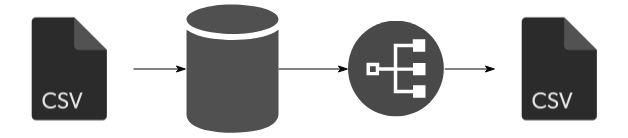
\includegraphics[scale=0.35]{./resources/figures/analysis.png}
    \end{mdframed}
    \caption[Analysis Workflow]{\textbf{Figure \ref{fig-analysis-workflow}: Process of analysis}}
    \label{fig-analysis-workflow}
\end{figure}


\section{MapReduce Approach}


\section{Performing joins}
Initial attempts at joining the three entities - Grades with Benchmarks, and then Grades with Benchmarks with Events were attempted directly via MapReduce. This approach involved specifying the map function to always output a value of the same format for all three entities. This format is a tuple of 11 indexes - [0, 0, 0, 0, 0, 0, 0, 0, 0, 0, 0]; each of the 11 indexes correlate to a specific output attribute. In other words, i=0 contained Grade \%, i=1,2,3,4,etc. the percents for Benchmark data, and the last 2 indexes (i = 9, i = 10) indicate an event occurrence (from the Event data) in either the first semester (i[9] = 1, i[10] = 0) or the second semester (i[9] = 0, i[10] = 1).

During index calculation, CouchDB iterates through every database document, passing each document to the Map function. This Map function instantiates the output tuple ([0, 0, 0, 0, 0, 0, 0, 0, 0, 0, 0]) on every execution, and then depending on the value of the `type\_' attribute of the document (this attribute is added to every document prior to insertion to CouchDB), the map function alters the corresponding component of the tuple, before returning and adding the key:value set to the view index currently being built.

To further explain, if the document being processed by the map function is a ‘grade’ document, then the map function adjusts the value tuple to emit the grade percent – i.e. [percent, 0, 0, 0, 0, 0, 0, 0, 0, 0, 0]. Or if the document is of type benchmark, the map function changes the values at indexes 1 through 8 and emits the value: [0, x, x, x, x, x, x, x, x, 0, 0]. If the document is of type ‘event’, then the map function alters the value at indexes 9 and 10. i.e. [0, 0, 0, 0, 0, 0, 0, 0, s1Event, s2Event] (s1Event is 1 for first semester event, or 0 for second semester, etc.).

The reduce function (whether that is the \_stats function a used in this study or any other function) then receives a tuple of tuples (a list of the tuples output by the map function executions), as the output per key, and can perform calculations across corresponding indexes; i.e. a single key references up to 3 tuples: 1 Grade document output, 1 Benchmark document output, and 1 Event document output. By performing an aggregation across these tuples at corresponding indexes, the Grades percentage (i=0) is an aggregation of the grade as output from the Grade entity along with 0s, the Benchmark percentages are each aggregations of the Benchmark percent each along with 0s, and the Events data is an aggregation of event counts and 0s. As such, aggregation across the output tuple effectively only takes into account relevant values (since all other values are 0) and a join is achieved.

However, for this approach to work, the reduce function needs to be able to group by common keys. To perform a grouping on the compound key [Student ID, Course, Course Year], all the entities need to output data in this format; but the Events data doesn't include Course, and the the Benchmarks data doesn't include Course or Course Year. As such, to allow for Grade data to be joined to Benchmark data on Course and Course Year in addition to Student ID, each Benchmark document needs to be output for every possible combination of Course and Course Year per student. That is the same with the Events documents - each Event needs to be output for every possible course that a student took in a given year.

In terms of performance this approach is disastrous. To analyze 40 courses taken over 3 years, each Benchmark document needs to be emitted for a student $40 x 3 = 120$ times so that the key of the Grade document [Student ID, Course, Year] can always be joined to Benchmark document. Likewise, Each Event data (which has year but not course information) needs to be emitted 40 times - once for each course a join could potentially be performed on. Considering the large number of event documents, this is impracticable. For this approach to be efficient, event documents would need to be aggregated prior to joining to minimize the number of times event data is replicated.

Instead, CouchDB's usage of B+trees as a means of sorting view indexes by keys is utilized to allow for joining the 3 documents in the final dataset. Figure \ref{fig-mapreduce-key-output} shows key output for all three entities in the form: [ID, Course, Year]. Documents that don't have properties for these fields emit 0 instead; resulting in a predictable key format of for each entity that is ordered:

\begin{itemize}
    \item \textit{benchmarks} document: [Id, 0, 0]
    \item \textit{events} document: [Id, 0, Year]
    \item \textit{grades} document: [ID, Course, Year]
    \item \textit{grades} document: [ID, Course, Year]
    \item etc...
\end{itemize}

Although many \textit{events} documents are outputted by the map function per student, due to reduction grouping all these documents by common key, only a single document that is an aggregation of all \textit{events} documents will be stored as reduced output in the view. So, for any student ID, scanning the index iteratively produces first a Benchmark document, then a single (aggregated) Event document, then a single Grade document for each course that student enrolled in. This results in a much more efficient way of aggregating different types of documents for a given set of keys. With ordered output, and Event data already aggregated via the reduce function, data retrieval involves iterating over view indexes, processing a single ID at a time. This is very efficient in terms of memory usage since only documents relating to a single ID need to be held in memory at a time - but the iteration has the potential to be much larger than it needs to be.

Filtering during map function execution cannot be done dynamically - that is, map and reduce function execution is isolated with database interactions during execution not possible. This is for security reasons, as well as the complications that could occur if a database's state could be changed by a map function during that map function's execution \cite{slack28Feb}. An experiment to implement the couchjs engine using Google's V8 engine (i.e. using node.js) was abandoned due the numerous APIs that extend JavaScript beyond the specification allowing network requests, file system access, etc. etc. \cite{v8couchjs, slack28Feb} making the map and reduce execution environment (for custom reduce function) insecure - as such, the experiment was abandoned in 2013.

\begin{figure}[H]
    \centering
    \begin{mdframed}
        \centering
        \begin{minted}{text}
// Map output
[<ID>, ‘0’, 1]: [0, b1, b2, b3, b4, b5, b6, b7, b8, 0, 0]
[<ID>, ‘0’, <Year>]: [0, 0, 0, 0, 0, 0, 0, 0, 0, 1, 0]
[<ID>, ‘0’, <Year>]: [0, 0, 0, 0, 0, 0, 0, 0, 0, 1, 0]
[<ID>, ‘0’, <Year>]: [0, 0, 0, 0, 0, 0, 0, 0, 0, 0, 1]
[<ID>, ‘0’, <Year>]: [0, 0, 0, 0, 0, 0, 0, 0, 0, 0, 1]
[<ID>, ‘0’, <Year>]: [0, 0, 0, 0, 0, 0, 0, 0, 0, 0, 1]
[<ID>, ‘0’, <Year>]: [0, 0, 0, 0, 0, 0, 0, 0, 0, 1, 0]
[<ID>, ‘CSC1015F’, <Year>]: [98, 0, 0, 0, 0, 0, 0, 0, 0, 0, 0]
[<ID>, ‘MAM100F, <Year>]: [94, 0, 0, 0, 0, 0, 0, 0, 0, 0, 0]

// Resulting reduce output
[<ID>, ‘0’, 1]: [0, b1, b2, b3, b4, b5, b6, b7, b8, 0, 0]
[<ID>, ‘0’, <Year>]: [0, 0, 0, 0, 0, 0, 0, 0, 0, 3, 3]
[<ID>, ‘CSC1015F’, <Year>]: [98, 0, 0, 0, 0, 0, 0, 0, 0, 0, 0]
[<ID>, ‘MAM100F, <Year>]: [94, 0, 0, 0, 0, 0, 0, 0, 0, 0, 0]
        \end{minted}
    \end{mdframed}
    \caption[Aggregation By Sorted MapReduce output]{\textbf{Figure \ref{fig-mapreduce-key-output}: \textit{map} and \textit{reduce} function output}
    \label{fig-mapreduce-key-output}
\end{figure}
